%\vskip -27.7pt
\begin{IEEEbiography}
[{\includegraphics[width=1in,height=1.25in,clip,keepaspectratio]{./photos/Chunfeng_Liu}}] 
{Chunfeng Liu} 
received the bachelor degree in automation from Tsinghua University, Beijing,
China, in 2009 and the master degree in microelectronics from Tsinghua
University, Beijing, China, in 2015. He is currently a PhD student with the Chair
of Electronic Design Automation, Technical University of Munich (TUM). His research interests focus on
computer-aided design for microfluidic biochips. 
\end{IEEEbiography}
\vskip -27.7pt
\begin{IEEEbiography}
[{\includegraphics[width=1in,height=1.25in,clip,keepaspectratio]{./photos/Xing}}] 
{Xing Huang} 
Xing Huang received the B.S. degree in computer science and technology 
and the Ph.D. degree in electronic science and technology from Fuzhou University, Fuzhou, China, in 2013 and 2018, respectively. 
From 2016 to 2017, he was a joint Ph.D. with the Department of Electrical and Computer Engineering, Duke University, Durham, NC, USA, 
supported by the Chinese Scholarship Council. 
From 2018 to 2019, he was a  Postdoctoral Research Fellow with the Department of Computer Science, National Tsing Hua University, Hsinchu, Taiwan.   
He is currently a Postdoctoral Research Fellow with the the Chair of Electronic Design Automation, Technical University of Munich, Germany. 
His current research interests include design automation for microfluidic biochips and integrated circuits.
\end{IEEEbiography}
\vskip -27.7pt
\begin{IEEEbiography}
[{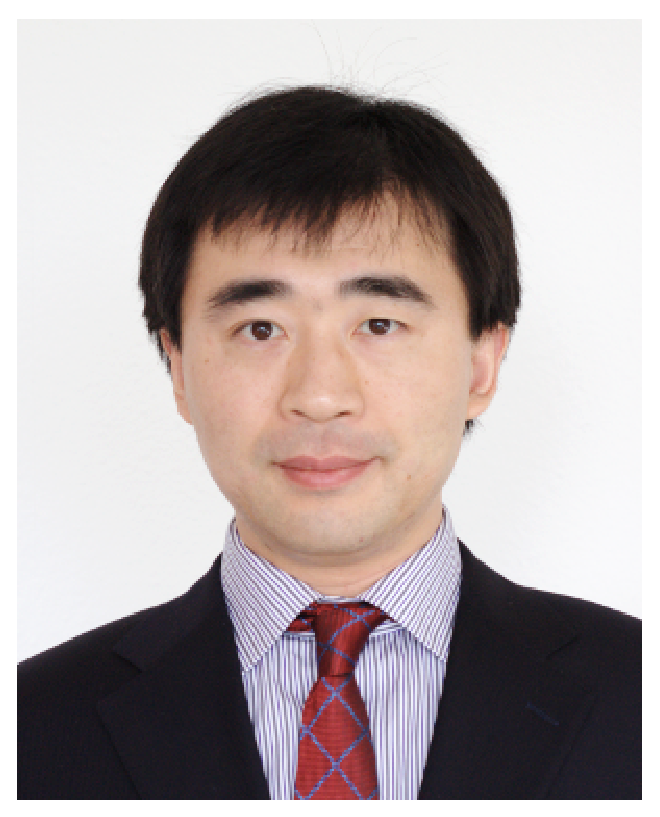
\includegraphics[width=1in,height=1.25in,clip,keepaspectratio]{./photos/Bing_Li}}] 
{Bing Li} 
Bing Li received the Dr.-Ing. degree from Technical University of Munich
(TUM), Munich, Germany, in 2010 and finished the Habilitation there in 2018.
He is currently a researcher with the Chair of Electronic Design Automation,
TUM. His research interests include high-performance and low-power
design of integrated circuits and systems. He has served on the Technical
Program Committees of several conferences including ICCAD, DATE, ASP-
DAC, etc.
\end{IEEEbiography}

\vskip -27.7pt
\begin{IEEEbiography}
[{\includegraphics[width=1in,height=1.25in,clip,keepaspectratio]{./photos/hailong}}] 
{Hailong Yao} 
Hailong Yao (SM’15) received the B.S. degree in computer science and technology from Tianjin University, Tianjin, China, in 2002, and the Ph.D. degree in computer science and technology from Tsinghua University, Beijing, China, in 2007.
From 2007 to 2009, he was a Post-Doctoral Research Scholar with the Department of Computer Science and Engineering, University of California at San Diego, La Jolla, CA, USA. He joined the Department of Computer Science and Technology, Tsinghua University, as an Assistant Professor in 2009. His current research interests include computer-aided design for microfluidic biochips and very large scale integration physical design.
Dr. Yao was a recipient of two Best Paper Award Nominations at ICCAD in 2006 and 2008, respectively, the ISQED Best Paper Award Nomination in 2011, and the SASIMI Best Paper Award in 2016.
\end{IEEEbiography}

\vskip -27.7pt
\begin{IEEEbiography}
[{\includegraphics[width=1in,height=1.25in,clip,keepaspectratio]{./photos/paul_pop}}] 
{Paul Pop} 
received the Ph.D. degree in com-
puter systems from Linköping University, in 2003.
He is currently a Professor with DTU Compute,
Technical University of Denmark (DTU), and
the Director of the DTU’s IoT Research Center.
His main research interests include system-level
design of cyber-physical systems. He has pub-
lished extensively in this area. He received
the EDAA Outstanding Dissertations Award
(Co-Supervisor), in 2011, and the Best Paper
Award at the DATE 2005, RTiS 2007, CASES 2009, MECO 2013, and DSD
2016 conferences.
\end{IEEEbiography}
\vskip -27.7pt
\begin{IEEEbiography}
[{\includegraphics[width=1in,height=1.25in,clip,keepaspectratio]{./photos/Tsungyi}}] 
{Tsung-Yi Ho} (M'08--SM'12) received his Ph.D. degree in Electrical Engineering from National Taiwan
University, Taipei, Taiwan, in 2005.  He is a Professor with the Department of Computer 
Science of National Tsing Hua University, Hsinchu, Taiwan. His research interests include 
design automation and test for microfluidic biochips and nanometer integrated circuits.
Dr. Ho was a recipient of the Best Paper Awards at the VLSI Test Symposium (VTS) in 2013 and IEEE
TCAD in 2015. Currently he serves as an ACM Distinguished Speaker, 
a Distinguished Lecturer of the IEEE Circuits and
Systems Society, and Associate Editor of the ACM JETC, ACM TODAES,
ACM TECS, and IEEE TVLSI, and the Technical Program Committees of
major conferences, including DAC, ICCAD, DATE, ASP-DAC, ISPD, etc.
\end{IEEEbiography}
\vskip -27.7pt
\begin{IEEEbiography}
[{
\includegraphics[width=1in,height=1.25in,clip,keepaspectratio]{./photos/Ulf_Schlichtmann}}] 
{Ulf Schlichtmann} (S'88--M'90--SM'18) received the Dipl.-Ing. and Dr.-Ing.
degrees in electrical engineering and information technology from Technical
University  of  Munich (TUM), Munich, Germany, in 1990 and 1995,  respectively.

He is Professor and the Head of the Chair of Electronic Design Automation at
TUM. He joined TUM in 2003, following 10 years in industry. His current
research interests include computer-aided design of electronic circuits and
systems, with an emphasis on designing reliable and robust systems.
Increasingly, he focuses on emerging technologies such as lab-on-chip and
photonics.
\end{IEEEbiography}

\vfill

